%!TEX program = xelatex
% 完整编译: xelatex -> biber/bibtex -> xelatex -> xelatex
\documentclass[lang=cn,11pt,a4paper]{elegantpaper}

\title{网格生成的简短报告}
\author{W Huang}
\date{\zhtoday}


% 本文档命令
\usepackage{array}
\usepackage{float}
\usepackage{multirow}
\newcommand{\ccr}[1]{\makecell{{\color{#1}\rule{1cm}{1cm}}}}

\begin{document}

\maketitle

\section{deal.II的网格生成}

在deal.II的用户手册中,展示了这样的一类网格:

\begin{figure}[H]
    \centering
    \begin{minipage}[t]{0.45\textwidth}
        \centering
        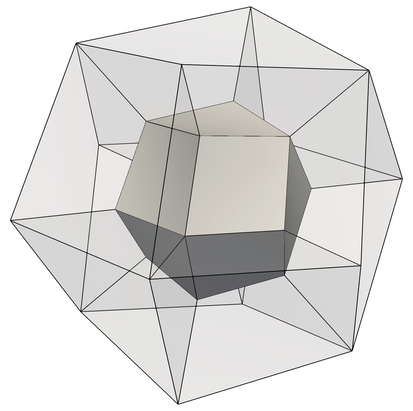
\includegraphics[width=0.5\textwidth]{png/hypershell3d-12.png}
    \end{minipage}
    \begin{minipage}[t]{0.45\textwidth}
        \centering
        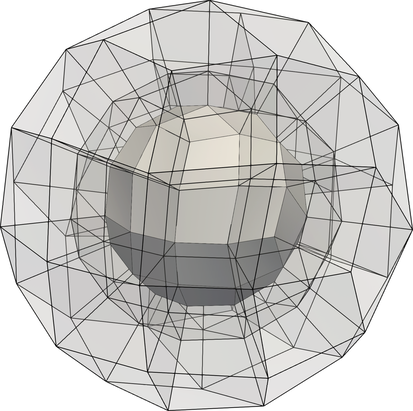
\includegraphics[width=0.5\textwidth]{png/hypershell3d-96.png}
    \end{minipage}
\end{figure}

设$n$表示Volume的个数,这类网格只支持特定的几个$n$。左图结构并非算法生成,而是手工绘制的,然后根据用户输入的内外球壳半径来伸缩,右图是左图经过一次细化得到。

我们可能需要\textbf{手工绘制}立方体挖球的网格,只需要一个粗的网格,deal.II可以自动细化。

另外,对于复杂几何区域,deal.II的Tutorial似乎是推荐用gmsh先生成一个粗网格。但我试了一下gmsh,生成的六面体网格极其丑陋。
\begin{figure}[H]
    \centering
    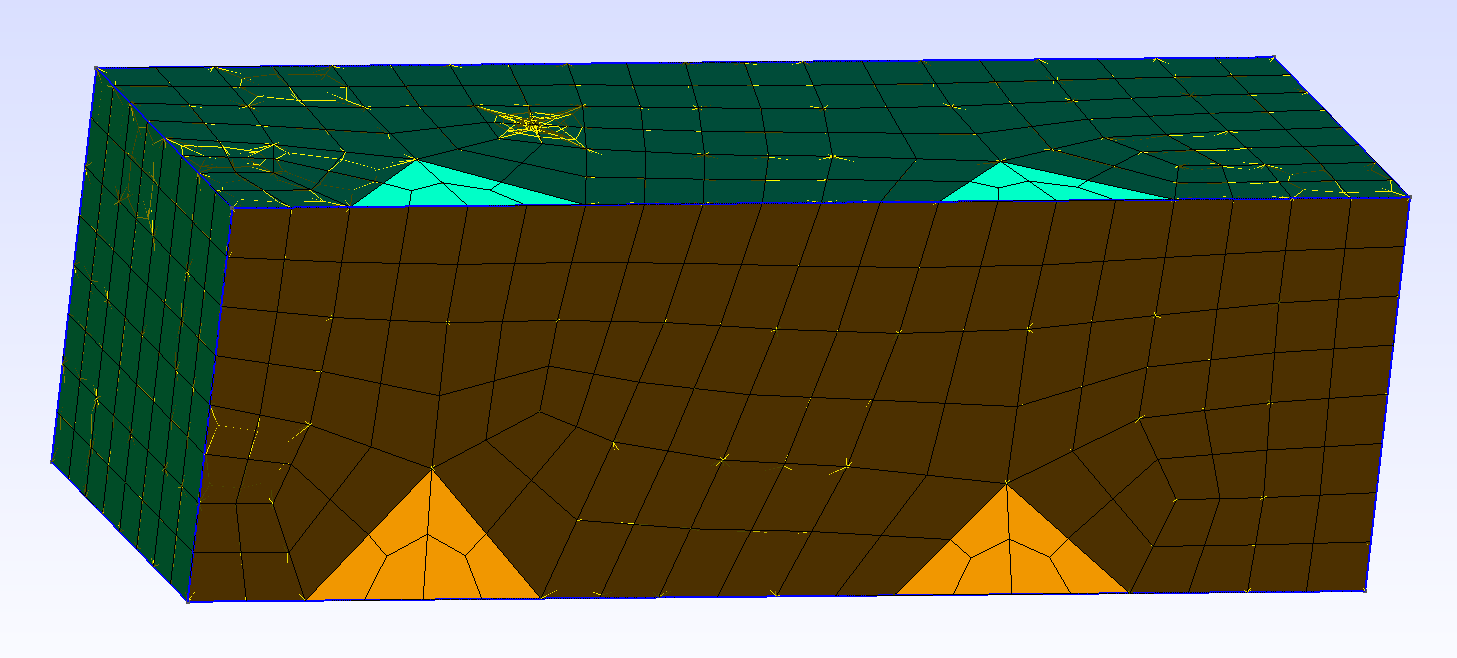
\includegraphics[width=0.6\textwidth]{png/3d-face.png}
    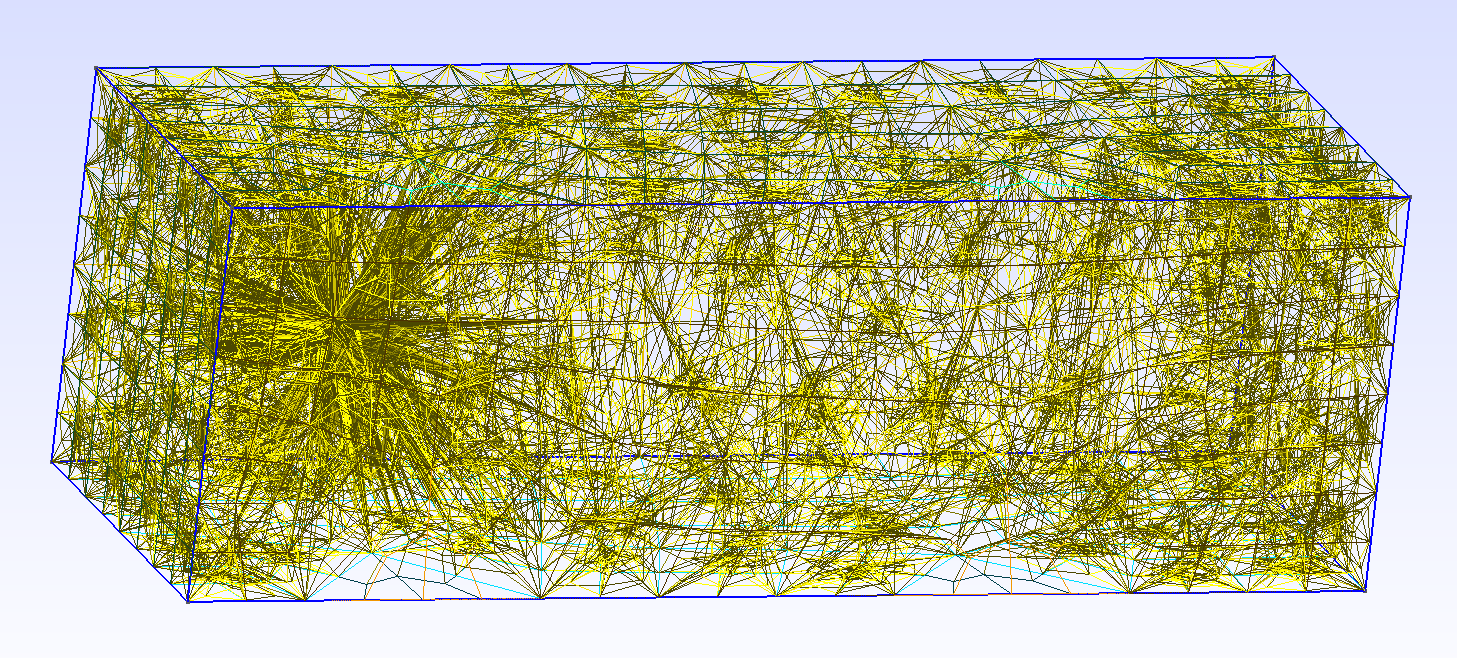
\includegraphics[width=0.6\textwidth]{png/3d-inner.png}
\end{figure}

gmsh只有在每一层横截面都一样的几何结构中,才能生成好看的网格,例如下图。
\begin{figure}[H]
    \centering
    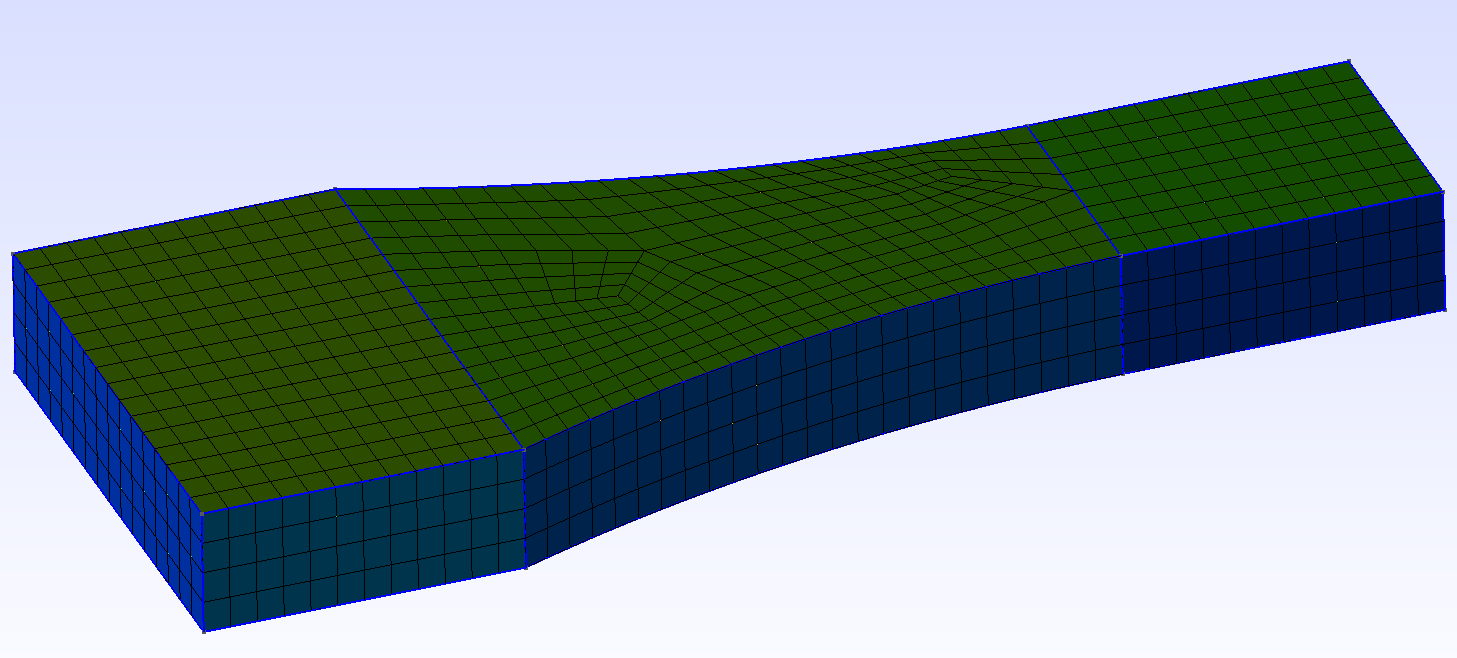
\includegraphics[width=0.6\textwidth]{png/3d-nice.png}
\end{figure}

\textbf{upd. Oct. 24.} 在deal.II里没有找到自动生成3维任意区域网格的接口。还是需要gmsh。但gmsh的算法是先生成边界上的二维网格,然后再生成内部的三维网格,所以立方体里挖掉一个球的时候,边界网格差异太大了,它的算法没法生成好看的内部网格。

\begin{figure}[H]
    \centering
    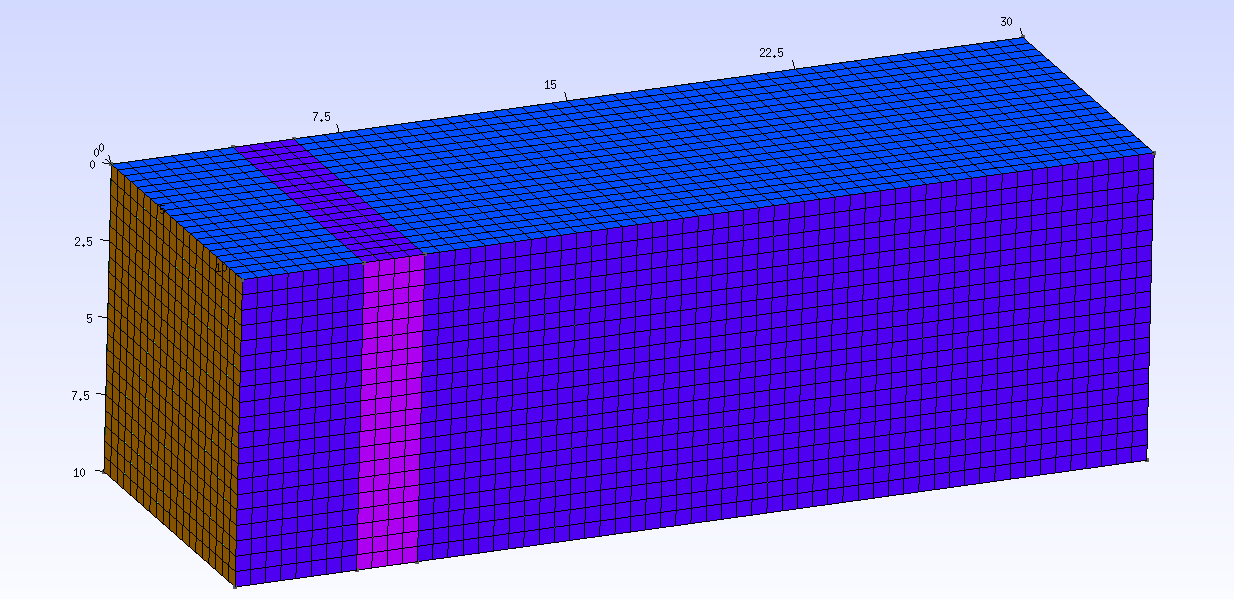
\includegraphics[width=0.6\textwidth]{png/outer.png}
    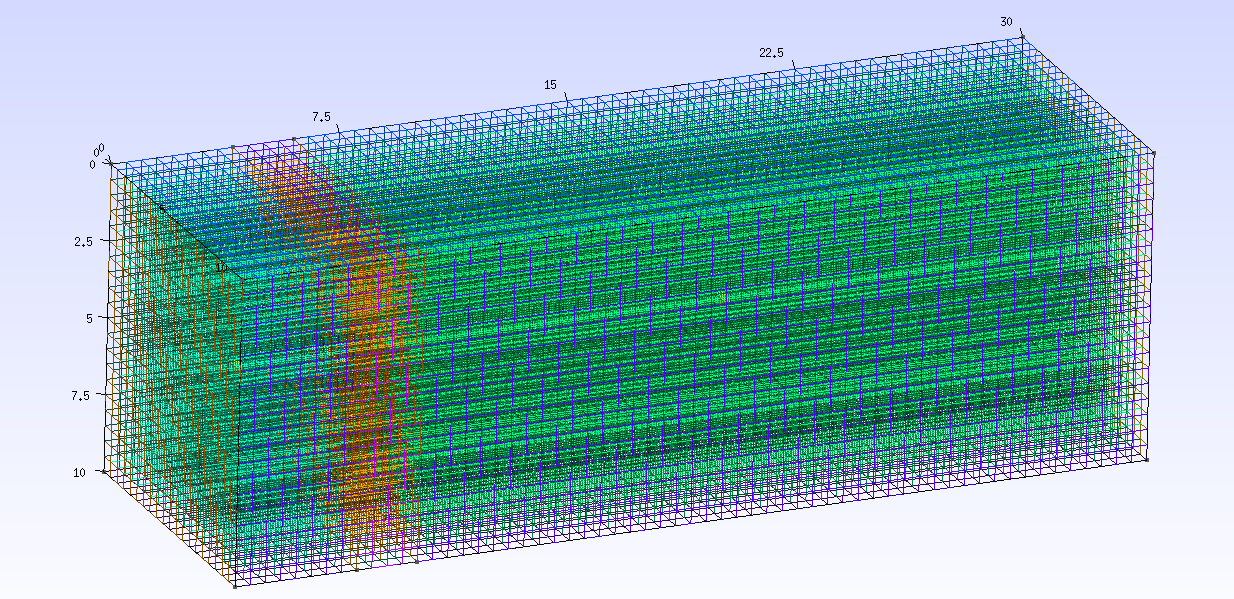
\includegraphics[width=0.6\textwidth]{png/outer-volume.png}
    \caption{外网格:长方体里挖掉一个正方体,网格很漂亮}
    \begin{minipage}[t]{0.45\textwidth}
        \centering
        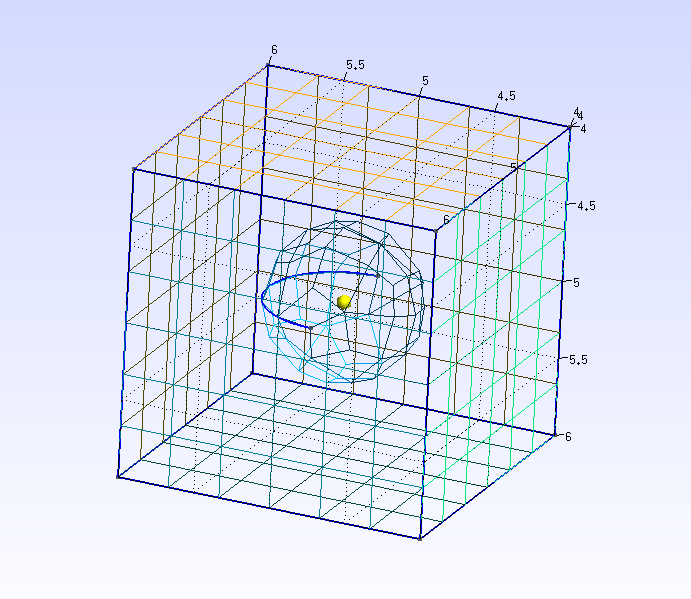
\includegraphics[width=0.8\textwidth]{png/inner.png}
    \end{minipage}
    \begin{minipage}[t]{0.45\textwidth}
        \centering
        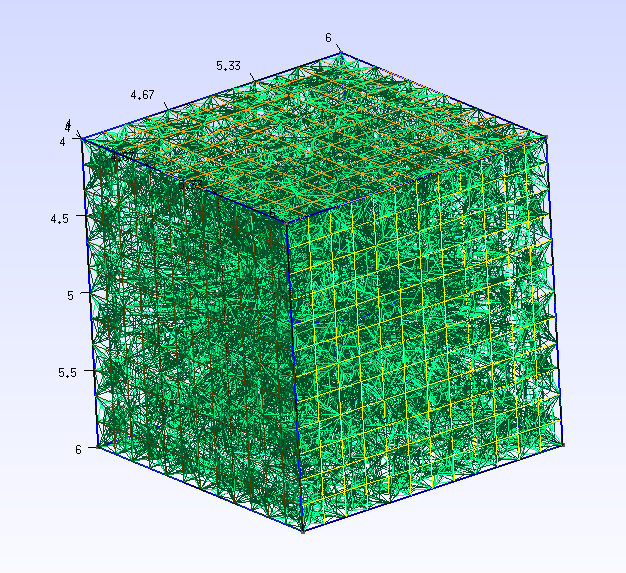
\includegraphics[width=0.8\textwidth]{png/inner-volume.png}
    \end{minipage}
    \caption{内网格:正方体里挖掉一个球(边界网格好看,内部bullshit)}
\end{figure}

我想把内外网格合并起来,但内网格太丑了,怎么办呢?

\appendix
%\appendixpage
\addappheadtotoc

\end{document}
